\documentclass{article}
\usepackage[T1]{fontenc}
\usepackage{lmodern}
\usepackage{graphicx}
\usepackage{amsmath,amssymb}
\usepackage[a4paper,margin=2cm]{geometry}
\usepackage[absolute,overlay]{textpos}
\setlength{\TPHorizModule}{1mm}
\setlength{\TPVertModule}{1mm}
\usepackage[indonesian]{babel}
\usepackage{hyperref}
\setlength{\emergencystretch}{2em}
% unit: Halaman 44

\begin{document}

% === Halaman 44 (python/native) ===

44

• Kriptanalisis (cryptanalysis): ilmu dan seni untuk memecahkan chiperteks 

menjadi plainteks tanpa mengetahui kunci yang digunakan. 

• Pelakunya disebut kriptanalis

• Kriptanalisis merupakan “lawan” kriptografi

• Teknik kriptanalisis sudah ada sejak abad ke-9. 

Kriptanalisis dikemukakan pertama kali oleh 

seorang ilmuwan Arab pada Abad IX  bernama 

Abu Yusuf Yaqub Ibnu Ishaq Ibnu As-Sabbah 

Ibnu 'Omran Ibnu Ismail Al-Kindi, atau yang 

lebih dikenal sebagai Al-Kindi. 

Al-Kindi depicted in a Syrian Post stamp.

Kriptanalisis

% deskripsi: gambar native xref 223
\noindent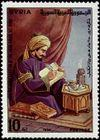
\includegraphics[width=0.85\textwidth]{../../images/python/page_044_img_01.jpeg}

\end{document}
